% ============================================================
% Chapter 7 --- Connectedness
% Originally: content/week-03.tex, \section{Connectedness} (Corsin Week 3, Monday) and
%             \section{Path connectedness} (Corsin Week 3, Friday)
% ============================================================
\chapter{Connectedness}
\label{ch:connectedness}

% Transition: Claude Opus 5 (Medium)
Compactness told us when a space has \qt{enough finiteness} to guarantee extrema and uniform
behaviour. This chapter turns to a completely different, qualitative kind of structure: whether a
space can be split into separate pieces at all. Connectedness and path connectedness are the two
answers, they are not equivalent, and the topologist's sine curve is the standard witness.

% Originally: content/week-03.tex, \section{Connectedness} (Corsin Week 3, Monday)

\section{Connectedness}
\label{sec:connectedness}

\begin{definition}[Connected and disconnected metric spaces]
\label{def:connectedness}
A metric space $(X,d)$ is \newterm{disconnected} (\germanterm{unzusammenh\"angend}) if there
exist $U_1, U_2 \subseteq X$ subsets which are
\begin{enumerate}[label=\textbf{(\alph*)}]
  \item \textbf{open},
  \item \textbf{non-empty}, $U_1 \neq \emptyset \neq U_2$,
  \item \textbf{disjoint}, $U_1 \cap U_2 = \emptyset$,
\end{enumerate}
such that $X = U_1 \cup U_2$. Similarly, for a subset $A \subseteq X$, it is disconnected if it is
disconnected as a metric space with the induced metric $d|_{A \times A}$. \newterm{Connected}
(\germanterm{zusammenh\"angend}) is the negation of disconnected.
\end{definition}

Typically, proving that a set or metric space is connected is done \textbf{by contradiction},
which is why one should remember the definition of \textit{disconnected}. Intuitively, connected
means: \qt{the space cannot be separated by open sets.}

\begin{center}
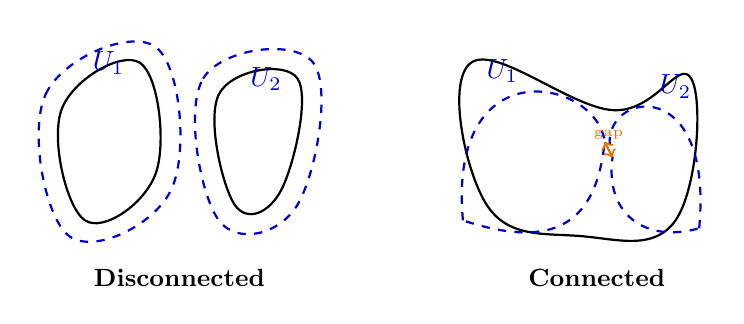
\begin{tikzpicture}[scale=1.0]
  % Left panel: Disconnected
  \begin{scope}[shift={(0,0)}]
    \draw[thick] plot[smooth cycle, tension=0.7] coordinates {(-1.5,-0.8) (-1.8,0.6) (-0.8,1.2) (-0.6,-0.2)};
    \draw[thick] plot[smooth cycle, tension=0.7] coordinates {(0.4,-0.6) (0.2,0.8) (1.2,1.0) (1.0,-0.4)};

    \draw[blue!80!black, thick, dashed] plot[smooth cycle, tension=0.7] coordinates {(-1.7,-1.0) (-2.0,0.8) (-0.6,1.4) (-0.4,-0.4)};
    \node[blue!80!black] at (-1.2,1.2) {$U_1$};

    \draw[blue!80!black, thick, dashed] plot[smooth cycle, tension=0.7] coordinates {(0.2,-0.8) (0.0,1.0) (1.4,1.2) (1.2,-0.6)};
    \node[blue!80!black] at (0.8,1.0) {$U_2$};

    \node[below, font=\small] at (-0.3,-1.3) {\textbf{Disconnected}};
  \end{scope}

  % Right panel: Connected
  \begin{scope}[shift={(5.0,0)}]
    \draw[thick] plot[smooth cycle, tension=0.7] coordinates {(-1.4,-0.6) (-1.6,1.2) (0.2,0.6) (1.2,1.0) (1.0,-0.8) (-0.2,-1.0)};

    \draw[blue!80!black, thick, dashed] (-1.7,-0.8).. controls (-1.9,1.4) and (0.0,1.0).. (0.1,0.2).. controls (0.0,-0.8) and (-0.5,-1.2).. (-1.7,-0.8);
    \node[blue!80!black] at (-1.2,1.1) {$U_1$};

    \draw[blue!80!black, thick, dashed] (1.3,-0.9).. controls (1.5,1.2) and (-0.1,0.8).. (0.2,0.0).. controls (0.1,-0.7) and (0.6,-1.1).. (1.3,-0.9);
    \node[blue!80!black] at (1.0,0.9) {$U_2$};

    \draw[orange!90!black, <->, thick] (0.1,0.2) -- node[above, font=\tiny] {gap} (0.2,0.0);

    \node[below, font=\small] at (0,-1.3) {\textbf{Connected}};
  \end{scope}
\end{tikzpicture}
\end{center}

% Generator: Claude Opus 5 (High) --- the base case of connectedness, used three times in this
% chapter (path-connectedness, the topologist's sine curve, the intermediate value theorem)
% but stated nowhere in the source notes.
\begin{proposition}[Intervals are connected]
\label{prop:intervals_connected}
Every interval $I \subseteq \mathbb{R}$ --- open, closed, half-open, bounded or not --- is
connected (\cref{def:connectedness}). Conversely, a connected subset of $\mathbb{R}$ is an
interval.
\end{proposition}

\begin{proof}
Suppose $I = U_1 \sqcup U_2$ with $U_1, U_2$ open in $I$, disjoint and both non-empty. Pick
$a \in U_1$ and $b \in U_2$; without loss of generality $a<b$, and $[a,b] \subseteq I$ because
$I$ is an interval. Set
\[c := \sup\{\,t \in [a,b] \ :\ [a,t] \subseteq U_1\,\},\]
which is well defined since $a$ belongs to the set. Now $c \in [a,b] \subseteq I$, so $c$ lies
in $U_1$ or in $U_2$, and both lead to a contradiction:
\begin{itemize}
  \item If $c \in U_1$, openness gives $\varepsilon>0$ with $(c-\varepsilon,c+\varepsilon)\cap I
    \subseteq U_1$; together with $[a,c) \subseteq U_1$ this yields $[a,t] \subseteq U_1$ for
    some $t>c$ unless $c=b$ --- contradicting either the supremum or $b \in U_2$.
  \item If $c \in U_2$, openness gives $\varepsilon>0$ with $(c-\varepsilon,c] \cap I \subseteq
    U_2$. But $c>a$ (as $a \in U_1$ is open in $I$), so by definition of the supremum there is
    $t \in (c-\varepsilon,c]$ with $[a,t] \subseteq U_1$ --- contradicting disjointness.
\end{itemize}
So no such splitting exists, and $I$ is connected. For the converse, a set $A \subseteq
\mathbb{R}$ that is not an interval admits $a<c<b$ with $a,b \in A$ and $c \notin A$; then
$A \cap (-\infty,c)$ and $A \cap (c,\infty)$ disconnect it.
\end{proof}

\begin{remark}[Why this is the only example one ever needs]
\label{rem:intervals_are_the_base_case}
Every connectedness proof in this chapter reduces to \cref{prop:intervals_connected}: a path is
a continuous image of $[0,1]$ (\cref{def:path}), so path-connected sets are connected
(\cref{lem:path_connected_implies_connected}) purely because the \emph{interval} is; and the
intermediate value theorem, invoked in the topologist's sine curve below, is
\cref{thm:continuity_preserves_connected} applied to an interval, since the connected subsets of
$\mathbb{R}$ are exactly the intervals. In other words, the single fact that $\mathbb{R}$ has no
gaps --- the completeness axiom, which is what powers the supremum above --- is the source of
all of it.
\end{remark}

\begin{aiexample}[Disconnectedness of Rational Numbers]
% Generator: Gemini 3.6 Flash (Medium)
The set of rational numbers $\mathbb{Q} \subset \mathbb{R}$ equipped with the subspace topology is disconnected. To see this, define
\[
U := \mathbb{Q} \cap (-\infty, \sqrt{2}) \quad \text{and} \quad V := \mathbb{Q} \cap (\sqrt{2}, \infty).
\]
Since $\sqrt{2} \notin \mathbb{Q}$, we have $U \cup V = \mathbb{Q}$ and $U \cap V = \emptyset$. Both $U$ and $V$ are non-empty and open in the subspace topology of $\mathbb{Q}$ (as intersections of $\mathbb{Q}$ with open intervals in $\mathbb{R}$). Hence $U$ and $V$ form a separation of $\mathbb{Q}$.
\end{aiexample}

% Supplement: Sascha Brack/Class Notes/Week_02_Notes_Friday_Updated.pdf, p. 9
\begin{example}[A disconnected set in $\mathbb{R}^2$]
Let $X := ([0,1] \times [0,1]) \cup ([2,3] \times \{1\}) \subseteq \mathbb{R}^2$. Is $X$ connected?
No. Let $U := \{(x,y) \in X \mid x < 1.5\}$ and $V := \{(x,y) \in X \mid x > 1.5\}$. We can write these as $U = X \cap \{(x,y) \in \mathbb{R}^2 \mid x < 1.5\}$ and $V = X \cap \{(x,y) \in \mathbb{R}^2 \mid x > 1.5\}$. Both $U$ and $V$ are open in the subspace topology of $X$ because they are intersections of $X$ with open half-planes in $\mathbb{R}^2$. Furthermore, $X = U \cup V$, and $U, V$ are disjoint and non-empty. Thus, $X$ is disconnected.
\begin{center}
\begin{tikzpicture}[scale=1.5]
  \draw[->, thick] (-0.2,0) -- (3.5,0);
  \draw[->, thick] (0,-0.2) -- (0,1.5);
  
  \draw[very thick, fill=purple!20, pattern=north east lines, pattern color=purple] (0,0) rectangle (1,1);
  \draw[very thick, purple] (2,1) -- (3,1);
  \node[purple, left] at (-0.1, 0.5) {$X$};
  
  \draw[green!60!black, dashed] (0.5, 0.5) circle (0.8);
  \node[green!60!black] at (1.2, 0.6) {$U$};
  
  \draw[green!60!black, dashed] (2.5, 1) ellipse (0.7 and 0.3);
  \node[green!60!black] at (2.5, 1.4) {$V$};
\end{tikzpicture}
\end{center}
\end{example}

\begin{theorem}[Continuous functions preserve connectedness]
\label{thm:continuity_preserves_connected}
Let $X$, $Y$ be metric spaces, $f : X \to Y$ continuous. If $A \subseteq X$ is connected, then
$f(A)$ is connected.
\end{theorem}

% Generator: Claude Opus 5 (High) --- stated without proof in the source; the argument is three
% lines and is the exact dual of \cref{item:continuity_preserves_compact}.
\begin{proof}
We may assume $A = X$, replacing $X$ by $A$ with the induced metric and $Y$ by $f(A)$. Suppose
$f(X)$ were disconnected, say $f(X) = V_1 \sqcup V_2$ with $V_1,V_2$ open in $f(X)$, disjoint
and non-empty. Then $U_i := f^{-1}(V_i)$ is open by \cref{def:continuous}\textbf{(c)},
non-empty because $V_i$ meets the image, and $U_1 \cap U_2 = \emptyset$ with
$U_1 \cup U_2 = X$ because the $V_i$ partition $f(X)$. So $U_1,U_2$ disconnect $X$, contrary to
hypothesis.
\end{proof}

\begin{corollary}[Intermediate value theorem]
\label{cor:intermediate_value_theorem}
Let $f : [a,b] \to \mathbb{R}$ be continuous. Then $f$ attains every value between $f(a)$ and
$f(b)$.
\end{corollary}

\begin{proof}
By \cref{prop:intervals_connected}, $[a,b]$ is connected, so $f([a,b])$ is connected by
\cref{thm:continuity_preserves_connected}, hence is an interval (\cref{prop:intervals_connected}
again). An interval containing $f(a)$ and $f(b)$ contains everything between them.
\end{proof}

\begin{ainote}
The intermediate value theorem is a result from \emph{Analysis I}, but it is worth re-deriving
it here in one line: it is the first place where connectedness earns its keep, and the proof
makes visible that the theorem is really a statement about $\mathbb{R}$ having no gaps rather
than about $f$. It is used in the topologist's sine curve
(\cpageref{ex:topologists_sine_curve}) below.
\end{ainote}

% Supplement: Sascha Brack/Class Notes/Week_03_Notes_Monday.pdf, p. 4
\begin{corollary}[Linear maps preserve the unit cube]
\label{cor:linear_maps_unit_cube}
Given the $n$-dimensional unit cube $[0,1]^n \subset \mathbb{R}^n$, any linear map $L : \mathbb{R}^n \to \mathbb{R}^n$ maps $[0,1]^n$ to an $n$-dimensional parallelepiped. Since linear maps in Euclidean space are continuous, the image $L([0,1]^n)$ is connected. Furthermore, since $[0,1]^n$ is compact, $L([0,1]^n)$ is also compact.
\end{corollary}

\begin{exercise}[Properties of connectedness]
\label{ex:connectedness_tf}
Are the following true or false?
\begin{enumerate}[label=\textbf{(\alph*)}]
  \item The union of connected subsets with a common point is connected.
  \item The intersection of connected subsets is connected.
  % Not a first introduction -- \newterm/\germanterm for "closure" belong to
  % \cref{def:interior_closure_boundary}, so this is a plain back-reference.
  \item The closure (\cref{def:interior_closure_boundary}) of a connected subset is connected.
\end{enumerate}
\end{exercise}

% Kept inline: solved directly in Corsin Nick/Class Notes/Week 3.pdf, pp. 5--6.
\begin{exercisesolution}[Proof of \cref{ex:connectedness_tf}]
\textbf{(a) True.} \textit{Proof.} Let $X$ be a metric space, $V_1, V_2 \subseteq X$ connected,
and $x_0 \in V_1 \cap V_2$. Suppose $V_1 \cup V_2 \subseteq U_1 \cup U_2$ with
$U_1, U_2 \subseteq X$ open and disjoint. Assume without loss of generality $x_0 \in U_1$. Then
$U_1 \cap V_1 \neq \emptyset$ and $U_1 \cap V_2 \neq \emptyset$. So, since $V_1, V_2$ are
connected, $V_1 \cap U_2 = V_2 \cap U_2 = \emptyset$. Therefore
$(V_1 \cup V_2) \cap U_2 = \emptyset$ and $V_1 \cup V_2$ is connected.

\textbf{(b) False.} \textit{Counterexample:}
\[
X = \mathbb{R}^2, \quad U = [-1,1] \times \{0\}, \quad V = S^1 = \{x \in \mathbb{R}^2 : \|x\| = 1\},
\]
\[
U \cap V = \{(-1,0), (1,0)\}.
\]

\textbf{(c) True.} Suppose $X$ is a metric space, $A \subseteq X$ a subset with closure
$\overline{A}$. Suppose $U_1, U_2 \subseteq X$ are disjoint open sets covering $\overline{A}$, and
assume without loss of generality $\overline{A} \cap U_1 \neq \emptyset$. Then, since $U_1$ is
open, $A \cap U_1 \neq \emptyset$. By connectedness of $A$, $U_2 \cap A = \emptyset$, and since
$U_2$ is open, also $U_2 \cap \overline{A} = \emptyset$.
\end{exercisesolution}

\begin{ainote}
Corsin writes $\|x\| = R^2$ in the definition of $S^1$ above; it must be $\|x\| = 1$, as the
stated intersection $\{(\pm 1, 0)\}$ confirms. Corrected here.
\end{ainote}

\begin{center}
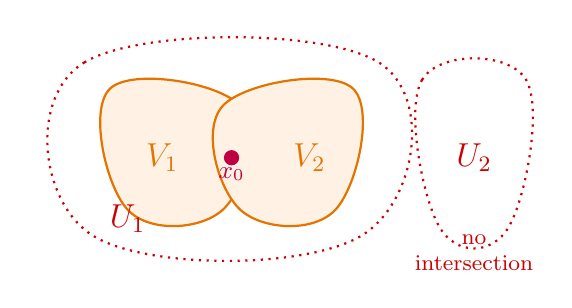
\begin{tikzpicture}[scale=1.1]
  \draw[orange!90!black, thick, fill=orange!10] plot[smooth cycle, tension=0.7] coordinates {(-1.6,-0.6) (-1.8,0.8) (-0.3,0.6) (-0.5,-0.6)};
  \node[orange!90!black, font=\large] at (-1.2,0) {$V_1$};

  \draw[orange!90!black, thick, fill=orange!10] plot[smooth cycle, tension=0.7] coordinates {(-0.3,-0.6) (-0.5,0.6) (1.0,0.8) (0.8,-0.6)};
  \node[orange!90!black, font=\large] at (0.5,0) {$V_2$};

  \fill[purple] (-0.4,0) circle (2.5pt) node[below, font=\small] {$x_0$};

  \draw[red!80!black, thick, dotted] plot[smooth cycle, tension=0.7] coordinates {(-2.0,-0.9) (-2.1,1.1) (1.3,1.1) (1.1,-0.9)};
  \node[red!80!black, font=\large] at (-1.6,-0.7) {$U_1$};

  \draw[red!80!black, thick, dotted] plot[smooth cycle, tension=0.7] coordinates {(2.0,-0.8) (1.8,0.9) (3.0,0.9) (2.8,-0.8)};
  \node[red!80!black, font=\large] at (2.4,0) {$U_2$};
  \node[red!80!black, font=\footnotesize, align=center] at (2.4,-1.1) {no\\intersection};
\end{tikzpicture}
\end{center}

\begin{center}
\begin{tikzpicture}[>=Latex, scale=1.3]
  \draw[->] (-1.6,0) -- (1.6,0) node[right] {$x$};
  \draw[->] (0,-1.6) -- (0,1.6) node[above] {$y$};

  \draw[red!80!black, thick] (0,0) circle (1.0);
  \node[red!80!black, above right] at (0.7,0.7) {$S^1$};

  \draw[orange!90!black, ultra thick] (-1,0) -- (1,0);
  \node[orange!90!black, below] at (0,-0.1) {$U = [-1,1]\times\{0\}$};

  \fill[purple] (-1,0) circle (2pt) node[above left, font=\footnotesize] {$(-1,0)$};
  \fill[purple] (1,0) circle (2pt) node[above right, font=\footnotesize] {$(1,0)$};
\end{tikzpicture}
\end{center}

% Originally: content/week-03.tex, \section{Path connectedness} (Corsin Week 3, Friday)

\section{Path connectedness}
\label{sec:path_connectedness}

% Transition: Claude Opus 5 (High)
\Cref{def:connectedness} defines connectedness negatively. A space is connected when it
\emph{cannot} be split, which is why proofs about it run by contradiction. That is mathematically
convenient and intuitively unsatisfying, since it says nothing whatever about what holds a
connected space together.

Path connectedness is the positive version, and it says the obvious thing: any two points can be
joined by a curve running inside the space. It implies connectedness
(\cref{lem:path_connected_implies_connected}), and on open subsets of $\mathbb{R}^n$ the two
notions agree (\cref{prop:open_euclidean_connected_path_connected}). In general they come apart,
and the topologist's sine curve at the end of this section is the standard witness.

% Source: Corsin Nick/Class Notes/Week 3.pdf, pp. 1--14
\begin{definition}[Path]
\label{def:path}
Let $(X,d)$ be a metric space. A continuous function $\gamma : [0,1] \to X$, where $[0,1]$
carries the standard metric, is called a \newterm{path} (\germanterm{Weg}). More generally, we
can replace $[0,1]$ by $[a,b]$ for $a < b$.
\end{definition}

\begin{definition}[Path-connected]
\label{def:path_connected}
A metric space $X$ (or subset thereof) is \newterm{path-connected}
(\germanterm{wegzusammenh\"angend}) if for all $x, y \in X$ there exists a path
(\cref{def:path}) $\gamma : [0,1] \to X$ with $\gamma(0) = x$, $\gamma(1) = y$.
\begin{center}
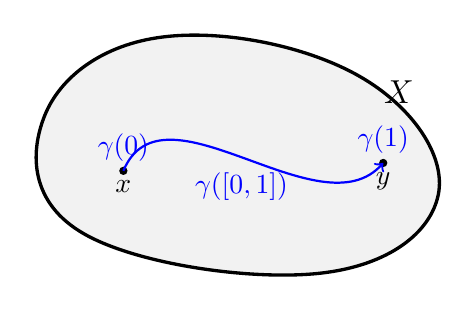
\begin{tikzpicture}
  \draw[very thick, fill=gray!10] plot[smooth cycle, tension=0.7] coordinates {(-2, -1) (-2.5, 0.5) (-1, 1.5) (1.5, 1) (2.5, -0.5) (1, -1.5)};
  \node[font=\large] at (2, 0.8) {$X$};
  
  \fill (-1.5, -0.2) circle (1.5pt) node[below] {$x$};
  \fill (1.8, -0.1) circle (1.5pt) node[below] {$y$};
  
  \draw[blue, thick, ->] (-1.5, -0.2) .. controls (-1, 1) and (1, -1) .. (1.8, -0.1);
  
  \node[blue, above] at (-1.5, -0.2) {$\gamma(0)$};
  \node[blue, above] at (1.8, -0.1) {$\gamma(1)$};
  \node[blue, below] at (0, -0.1) {$\gamma([0,1])$};
\end{tikzpicture}
\end{center}
\end{definition}

\begin{lemma}[Path-connected implies connected]
\label{lem:path_connected_implies_connected}
Let $X$ be a metric space. Then $X$ path-connected (\cref{def:path_connected}) implies $X$
connected (\cref{def:connectedness}).
\end{lemma}

% Generator: Claude Opus 5 (High) --- stated without proof in the source.
\begin{proof}
Suppose $X$ were path-connected but disconnected, say $X = U_1 \sqcup U_2$ with $U_1,U_2$ open,
disjoint and non-empty. Pick $x \in U_1$, $y \in U_2$ and a path $\gamma : [0,1] \to X$ with
$\gamma(0)=x$, $\gamma(1)=y$. Then $\gamma^{-1}(U_1)$ and $\gamma^{-1}(U_2)$ are open in $[0,1]$
by \cref{def:continuous}\textbf{(c)}, disjoint, cover $[0,1]$, and are non-empty (they contain
$0$ and $1$ respectively). This disconnects $[0,1]$, contradicting
\cref{prop:intervals_connected}.
\end{proof}

% Source: Jérôme Paschoud/Notizen/Woche 3.1 Banach und Kompaktheit.pdf, p. 6
% Generator: Gemini 3.6 Flash (High)
\begin{exercise}[The unit disk is connected]
\label{ex:disk_connected}
Prove that the set $S^1 := \{ (x,y) \in \mathbb{R}^2 \mid x^2 + y^2 \leq 1 \}$ is connected.
\end{exercise}

\begin{exercisesolution}[Proof of \cref{ex:disk_connected}]
Instead of proving connectedness directly via open sets, we can show that $S^1$ is path-connected, which implies connectedness (\cref{lem:path_connected_implies_connected}). Given any two points $a, b \in S^1$, we can connect them via a straight line segment. The segment can be parameterized as $\gamma(t) := (1-t)a + tb$ for $t \in [0,1]$. Since $S^1$ (the unit disk in $\mathbb{R}^2$) is convex, for any $t \in [0,1]$ we have $\lVert \gamma(t) \rVert \leq (1-t)\lVert a \rVert + t \lVert b \rVert \leq 1-t + t = 1$, so the entire path lies in $S^1$. Because any two points can be connected by a continuous path within $S^1$, the set is path-connected, and therefore connected.

(Note: The standard notation for the unit disk is $D^2$ or $B_1(0)$, whereas $S^1$ usually denotes the boundary circle $\{x^2+y^2=1\}$, but we reproduce the notation $S^1$ here as it appears in the source notes.)
\end{exercisesolution}

\begin{proposition}[Connectedness and path-connectedness in open Euclidean subsets]
\label{prop:open_euclidean_connected_path_connected}
Let $U \subseteq \mathbb{R}^n$ be open (\cref{def:open_closed}). Then
\[
U \text{ path-connected} \iff U \text{ connected}.
\]
\end{proposition}

% Generator: Claude Opus 5 (High) --- stated without proof in the source; the "(<=)" direction
% is the standard "the set of reachable points is clopen" argument and is worth having, since it
% is the only place in this chapter where openness is genuinely used.
\begin{proof}
\textbf{($\Rightarrow$)} is \cref{lem:path_connected_implies_connected}, which needs neither
openness nor $\mathbb{R}^n$.

\textbf{($\Leftarrow$)} Assume $U$ is connected and non-empty (the empty set is vacuously
path-connected), and fix $x_0 \in U$. Let
\[A := \{x \in U \ :\ \text{some path in } U \text{ joins } x_0 \text{ to } x\}.\]
We show $A$ and $U \setminus A$ are both open; since $x_0 \in A$ (take the constant path),
connectedness then forces $U\setminus A = \emptyset$, i.e.\ $A = U$, which is the claim.

Let $x \in U$ and choose $r>0$ with $B_r(x) \subseteq U$, using that $U$ is open. The ball is
convex, so every $y \in B_r(x)$ is joined to $x$ by the straight segment
$t \mapsto (1-t)x+ty$, which stays inside $B_r(x) \subseteq U$. Consequently:
\begin{itemize}
  \item If $x \in A$, concatenating a path from $x_0$ to $x$ with that segment joins $x_0$ to
    any $y \in B_r(x)$, so $B_r(x) \subseteq A$ and $A$ is open.
  \item If $x \notin A$, then no $y \in B_r(x)$ can lie in $A$, since otherwise running the
    segment backwards from $y$ to $x$ would join $x_0$ to $x$. So $B_r(x) \subseteq U\setminus A$ and
    $U\setminus A$ is open.
\end{itemize}
(Concatenation of two paths is again a path: traverse the first on $[0,\tfrac12]$ and the second
on $[\tfrac12,1]$, each at double speed; the result is continuous because the two pieces agree
at $t=\tfrac12$.)
\end{proof}

\begin{importantremark}[Only for open subsets]
\label{rem:path_connected_needs_open}
The implication \qt{connected $\Rightarrow$ path-connected} is \emph{false} without openness,
and the proof shows exactly why: the ball $B_r(x)$ around a point of $U$ was needed to supply
the straight segment. For a set that is not open there may be points with no room around them at
all, and the topologist's sine curve (\cref{ex:topologists_sine_curve}) below is precisely such
a case. There the origin has no neighbourhood in $S$ that is a nice piece of curve.
\end{importantremark}

% Source: Corsin Nick/Class Notes/Week 3.pdf, pp. 1--14
% (Re-cited: the two proofs and the important remark above are additions, not transcription.)
\begin{example}[The topologist's sine curve]
\label{ex:topologists_sine_curve}
\[S := \left\{\left(t, \sin\left(\tfrac{1}{t}\right)\right) : t > 0\right\} \cup \{(0,0)\} \subseteq \mathbb{R}^2\]
$S$ is \textbf{connected} but \textbf{not path-connected}!
\end{example}

\begin{ainote}
Corsin writes the second piece as $\cup\,\{0\}$; since $S \subseteq \mathbb{R}^2$, the point
being adjoined is the origin $(0,0) \in \mathbb{R}^2$, not the number $0$. Written as
$\cup\,\{(0,0)\}$ above, which is also what his own figure and the proof below use.
\end{ainote}

\begin{center}
\begin{tikzpicture}[>=Latex, scale=1.3]
  \draw[->] (-0.2,0) -- (3.2,0) node[right] {$t$};
  \draw[->] (0,-1.4) -- (0,1.4) node[above] {$y$};
  \draw (0,1.0) -- (-0.05,1.0) node[left, font=\footnotesize] {$1$};
  \draw (0,-1.0) -- (-0.05,-1.0) node[left, font=\footnotesize] {$-1$};
  % Horizontal figure-coordinate \x corresponds to t = \x/10, since the plot is sin(10/\x).
  \draw (1.0,0.05) -- (1.0,-0.05) node[below, font=\footnotesize] {$0.1$};
  \draw (2.0,0.05) -- (2.0,-0.05) node[below, font=\footnotesize] {$0.2$};

  \draw[blue!80!black, thick] plot[domain=0.08:2.8, samples=250] (\x, {sin((1.0/(\x*0.1)) r)});
  \fill[blue!80!black] (0,0) circle (1.5pt) node[left, font=\footnotesize] {$(0,0)$};
  \node[above, font=\small] at (1.5,1.3) {$S = \{(t, {\sin(1/t})) : t > 0\} \cup \{(0,0)\}$};
\end{tikzpicture}
\end{center}

\begin{proof}[$S$ is connected]
Write $G := S \setminus \{(0,0)\} = \{(t,\sin(1/t)) : t>0\}$ for the graph part, and suppose for
contradiction that $S$ is disconnected, say $S = V_1 \sqcup V_2$ with $V_1,V_2$ non-empty,
disjoint and open in $S$. Say $(0,0) \in V_1$.

$G$ is the continuous image of the interval $(0,\infty)$ under
$t \mapsto (t,\sin(1/t))$, hence path-connected, hence connected
(\cref{lem:path_connected_implies_connected}). A connected set meeting both parts of a
separation would itself be separated, so $G$ lies entirely in $V_1$ or entirely in $V_2$.

It cannot lie in $V_1$: then $V_2 \subseteq S \setminus (G \cup \{(0,0)\}) = \emptyset$,
contradicting $V_2 \neq \emptyset$. So $G \subseteq V_2$, and therefore
$V_1 = \{(0,0)\}$.

But $V_1$ is open in $S$, so some ball $B_\varepsilon\big((0,0)\big) \cap S$ equals
$\{(0,0)\}$, and that is false. For $t := \tfrac{1}{k\pi}$ with $k$ large, the point
$(t,\sin(1/t)) = (t,0) \in G$ lies within $\varepsilon$ of the origin. This is the required
contradiction, so $S$ is connected.
\end{proof}

\begin{proof}[$S$ is not path-connected]
Assume by contradiction there is a path from $(0,0)$ to $(\tfrac{1}{\pi}, 0)$,
\[
\gamma : [0,1] \to [0, \tfrac{1}{\pi}] \times [-1,1], \qquad t \mapsto (x(t), y(t)).
\]
Since $\gamma$ is continuous, $x$ and $y$ must also be continuous. By the \newterm{intermediate
value theorem} (\cref{cor:intermediate_value_theorem}), $x : [0,1] \to [0,\tfrac{1}{\pi}]$
attains every value in $[0,\tfrac{1}{\pi}]$, since $x(0) = 0$ and $x(1) = \tfrac{1}{\pi}$.
Therefore, we find a sequence $(a_n)_{n=1}^{\infty}$ such that
\[
x(a_n) = \frac{1}{2\pi n + \tfrac{\pi}{2}}.
\]
We may moreover choose the $a_n$ \textbf{decreasing}: having found $a_{n-1}$, apply the
intermediate value theorem on $[0,a_{n-1}]$ rather than on $[0,1]$, which is legitimate because
$x(0) = 0$ and $x(a_{n-1}) = \tfrac{1}{2\pi(n-1)+\pi/2}$ already straddle the next target value.
This yields $a_n \in (0,a_{n-1})$, so $(a_n)$ is decreasing and bounded below, hence convergent,
say $a_n \to \ell \in [0,1]$.

Now evaluate $\gamma$ along this sequence. By construction $x(a_n) \to 0$, so continuity gives
$x(\ell) = 0$; and $y(a_n) = \sin\!\big(2\pi n + \tfrac\pi2\big) = 1$ for every $n$, so
$y(\ell) = 1$. Hence $\gamma(\ell) = (0,1)$. But $(0,1) \notin S$: the only point of $S$ whose
first coordinate vanishes is the origin. This contradicts $\gamma([0,1]) \subseteq S$, so no
such path exists.
\end{proof}

\begin{ainote}
Corsin's argument produces the $a_n$ from the intermediate value theorem and then asserts
$a_n \to 0$. That does not follow from the choice as stated. The intermediate value theorem
returns \emph{some} preimage, and nothing so far prevents all of them from sitting near $1$.
The repair is the standard one and costs one sentence: apply the theorem on the shrinking
intervals $[0,a_{n-1}]$ rather than on $[0,1]$ each time, which forces the $a_n$ down. Inserted
above; the rest of his proof is unchanged.
\end{ainote}

\begin{center}
\begin{tikzpicture}[>=Latex, scale=1.3]
  \draw[->] (-0.3,0) -- (3.2,0) node[right] {$t$};
  \draw[->] (0,-1.4) -- (0,1.4) node[above] {$y$};

  \draw[blue!80!black, thick] plot[domain=0.08:2.8, samples=250] (\x, {sin((1.0/(\x*0.1)) r)});

  \fill[red!80!black] (0,0) circle (2pt) node[below left, font=\small] {$\gamma(0)$};

  % The peaks of the plotted sin(10/x) sit at x = 20/(pi(1+4k)), k = 1,2,3,...
  % -- these must land ON the curve, since they are the points gamma(a_n).
  \fill[red!80!black] (1.273,1.0) circle (2pt) node[above right, font=\footnotesize] {$\gamma(a_1)$};
  \fill[red!80!black] (0.707,1.0) circle (1.7pt);
  \fill[red!80!black] (0.490,1.0) circle (1.4pt);
  \fill[red!80!black] (0.374,1.0) circle (1.1pt);
  \fill[red!80!black] (0.303,1.0) circle (0.9pt);

  % The limit (0,1) is NOT a point of S -- hence the hollow circle.
  \draw[red!80!black, thick] (0,1.0) circle (2.5pt);
  \node[red!80!black, font=\footnotesize, left] at (-0.08,1.0) {$(0,1)$};
  \draw[red!80!black, ->, dashed] (1.15,1.19) -- (0.13,1.07);

  \node[red!80!black, font=\small] at (1.75,-1.15) {$\gamma(a_n) \to (0,1) \neq (0,0) = \gamma(0)$};
\end{tikzpicture}
\end{center}

% Sonnet 5 (Medium)
We close the week with a change of subject: away from topology and back to the linear-algebraic
structure (\cref{sec:structured_spaces}) that lets us talk about angles, not just distances.



% Originally: content/week-03.tex, end of \subsection{Contraction mappings}

\begin{aiexercise}[Continuous image of a path-connected set]
\label{ex:ai_connected_image}
% Generator: Claude Opus 5 (High). Replaces an earlier exercise asking for
% \cref{thm:continuity_preserves_connected}, which now carries its own proof.
Let $f \colon X \to Y$ be a continuous map between metric spaces.
\begin{enumerate}[label=\textbf{(\alph*)}]
  \item Prove that if $X$ is path-connected (\cref{def:path_connected}), then so is $f(X)$.
  \item Conclude that the graph $\Gamma_g := \{(x,g(x)) : x \in U\}$ of a continuous
    $g : U \to \mathbb{R}^m$ is path-connected whenever $U \subseteq \mathbb{R}^n$ is convex.
    (Compare \cref{ex:4.2}, which asks the same question with \qt{connected} in place
    of \qt{path-connected}.)
\end{enumerate}
\end{aiexercise}

% --- exercise relocated here from the dissolved sheet 4 ---

% Originally: content/week-04.tex, \exercisesheet{4}
% Source: exercises/Ex4_Analysis2_eng.pdf

\begin{exercise}[4.2 --- Connected graphs \textnormal{(important)}]
\label{ex:4.2}
Let $U \subset \mathbb{R}^n$ be open and connected and let $f \in C^1(U, \mathbb{R}^m)$. Show that
its graph
\[\Gamma_f := \{(x, f(x)) : x \in U\}\]
is a connected subset of $\mathbb{R}^n \times \mathbb{R}^m$.
\end{exercise}

% Originally: the \section{Solutions} of content/week-03.tex

\section{Solutions}
\label{sec:connectedness_solutions}

% Transition: Claude Opus 5 (High)
Not every solution in this chapter is collected here. \Cref{ex:connectedness_tf}
(\cpageref{ex:connectedness_tf}) and \cref{ex:disk_connected} (\cpageref{ex:disk_connected}) are
solved where they appear.

\begin{exercisesolution}[Proof of \cref{ex:ai_connected_image}]
% Generator: Claude Opus 5 (High)
\begin{enumerate}[label=\textbf{(\alph*)}]
  \item Let $p, q \in f(X)$, say $p = f(x)$ and $q = f(y)$. Since $X$ is path-connected there is
    a path $\gamma : [0,1] \to X$ with $\gamma(0)=x$ and $\gamma(1)=y$. Then
    $f \circ \gamma : [0,1] \to f(X)$ is continuous as a composition of continuous maps, and it
    satisfies $(f\circ\gamma)(0) = p$, $(f\circ\gamma)(1) = q$. So it is a path in $f(X)$ from
    $p$ to $q$, and $f(X)$ is path-connected.
  \item A convex set $U$ is path-connected: the straight segment $t \mapsto (1-t)x + ty$ lies in
    $U$ and is continuous. The map $\varphi : U \to \mathbb{R}^n\times\mathbb{R}^m$,
    $\varphi(x) := (x,g(x))$, is continuous because each component is, and
    $\Gamma_g = \varphi(U)$. Apply \textbf{(a)}.
\end{enumerate}

\begin{remark}
Part \textbf{(a)} is strictly easier than its connectedness counterpart
(\cref{thm:continuity_preserves_connected}), because path-connectedness is a statement one
verifies by \emph{exhibiting} something, namely a path, and continuous maps push paths forward
directly. Connectedness has no such witness to push forward, which is why its proof has to run
by contradiction through preimages instead. This asymmetry is worth noticing: it is the reason
path-connectedness is usually the easier of the two to prove, and connectedness the easier of
the two to \emph{use}.
\end{remark}
\end{exercisesolution}

% ===========================================================================
% Official sheet 3 (3.1--3.11). Derived independently, then checked against
% exercises/Sol3_Analysis2_eng.pdf.
% ===========================================================================

\begin{exercisesolution}[Proof of \cref{ex:4.2}]
% Generator: Claude Sonnet 5 (Medium)
Consider the map
\[
\varphi : U \to \mathbb{R}^n \times \mathbb{R}^m, \qquad x \mapsto (x, f(x)).
\]
Since $f \in C^1(U,\mathbb{R}^m)$ is in particular continuous, and the identity on $U$ is
continuous, $\varphi$ is continuous. By definition $\Gamma_f = \varphi(U)$. Since $U$ is connected
and $\varphi$ is continuous, \cref{thm:continuity_preserves_connected} gives that $\varphi(U) =
\Gamma_f$ is connected.
\end{exercisesolution}

\begin{exercisesolution}[Solution of \cref{ex:closed_unbounded_not_simply_connected}]
% Generator: Claude Opus 5 (High)
Take the closed exterior of the unit disc,
\[U := \{x \in \mathbb{R}^2 \mid \lvert x\rvert \ge 1\}.\]
\begin{itemize}
  \item \textbf{Closed:} $U$ is the preimage of the closed set $[1,\infty)$ under the continuous map
    $x \mapsto \lvert x\rvert$.
  \item \textbf{Unbounded:} it contains $(k,0)$ for every $k \in \mathbb{N}$.
  \item \textbf{Connected:} it is in fact path-connected. Given $p,q \in U$, travel radially outwards
    from $p$ to the circle of radius $R := \max\{\lvert p\rvert, \lvert q\rvert\}$, then along that
    circle, then radially inwards to $q$. Every point on this path has norm between $1$ and $R$, so
    the path stays in $U$.
  \item \textbf{Not simply connected:} the loop $\gamma(t) := (2\cos 2\pi t,\, 2\sin 2\pi t)$ winds
    once around the origin, and no loop with winding number $1$ about a point outside $U$ can be
    contracted to a point within $U$. Contracting it would force the loop to sweep across the
    removed open disc $\{\lvert x\rvert < 1\}$.
\end{itemize}
\begin{ainote}
The exercise is really a test of whether the three notions have been kept apart. Closed-and-unbounded
rules out the reflex answer of an annulus $\{1 \le \lvert x\rvert \le 2\}$, and \qt{connected but not
simply connected} rules out a half-plane or all of $\mathbb{R}^2$. Deleting an \emph{open} disc
rather than a point is what keeps the result closed while still puncturing it.
\end{ainote}
\end{exercisesolution}

\begin{exercisesolution}[Proof of \cref{ex:sphere_path_connected}]
% Generator: Claude Opus 5 (High)
Both directions are proved by looking at what $S^{n-1}$ actually is in the two cases.

\textbf{The case $n = 1$.} Here $S^0 = \{x \in \mathbb{R} \mid x^2 = 1\} = \{-1, +1\}$, a two-point
space. Suppose $\gamma : [0,1] \to S^0$ were a path with $\gamma(0) = -1$ and $\gamma(1) = 1$.
Regarded as a map into $\mathbb{R}$, it is continuous on an interval, so by the intermediate value
theorem it takes the value $0$ somewhere. But $0 \notin S^0$, a contradiction. Hence $S^0$ is not
path-connected.

\textbf{The case $n \ge 2$.} Fix $p, q \in S^{n-1}$, and suppose first that $q \neq -p$. Then the
straight segment between them misses the origin: if $(1-t)p + tq = 0$ for some $t \in [0,1]$, taking
norms gives $(1-t) = t$, so $t = \tfrac12$ and $p = -q$, which we excluded. We may therefore
normalise the segment and set
\[\gamma(t) := \frac{(1-t)p + tq}{\lvert (1-t)p + tq\rvert}, \qquad t \in [0,1].\]
This is continuous, takes values in $S^{n-1}$, and satisfies $\gamma(0) = p$, $\gamma(1) = q$.

It remains to handle $q = -p$, and this is exactly where $n \ge 2$ enters: the sphere $S^{n-1}$ then
contains a point $r$ with $r \neq \pm p$. (For $n \ge 2$ the sphere is infinite --- pick any unit
vector $v$ orthogonal to $p$, which exists because $p^\perp$ has dimension $n - 1 \ge 1$.) Neither
$r$ nor $q$ is the antipode of the other's partner, so the previous construction gives a path from
$p$ to $r$ and a path from $r$ to $q$; concatenating them joins $p$ to $q$. Hence $S^{n-1}$ is
path-connected.
\begin{remark}
The construction in the main case is the radial projection of the segment, and it is the standard way
to move around a sphere: it works verbatim on any $S^{n-1}$ and explains why the antipodal pair is
the only obstruction. Note also that $n \ge 2$ is used only once, to produce a third point --- which
is precisely what $S^0$ does not have.
\end{remark}
\begin{ainote}
The official solution introduces the same construction with the words \qt{now let $n \ge 1$}, and
then disposes of the antipodal case $x = -y$ by composing two paths through \qt{an arbitrary other
point $w \in S^{n-1}$}. For $n = 1$ there is no such $w$: $S^0 = \{\pm1\}$ consists of $x$ and $-x$
and nothing else. The bound is therefore $n \ge 2$, exactly as the statement being proved requires
--- and as the official solution's own preceding paragraph, which shows $S^0$ is \emph{not}
path-connected, confirms. The step is written out explicitly above rather than left to the reader,
since it is the only place the hypothesis is used.
\end{ainote}
\end{exercisesolution}

\begin{exercisesolution}[Proof of \cref{ex:examHS24_TF_topology}]
% Generator: Gemini 3.1 Pro (High)
\begin{enumerate}[label=\textbf{(\alph*)}]
  \item \textbf{True:} $U$ is defined by non-strict inequalities involving continuous functions (specifically, the pre-image of $[0, \infty)$ under $g_1(x,y) = y+x^2$ and $g_2(x,y) = x^2-y$). Consequently, $U$ is closed.
  \item \textbf{True:} We can contract $U$ to the origin via the homotopy $H((x,y), t) = (tx, t^2y)$ for $t \in [0,1]$. Note that $(tx)^2 = t^2x^2$, and since $-x^2 \le y \le x^2$, multiplying by $t^2 \ge 0$ gives $-(tx)^2 \le t^2y \le (tx)^2$, which ensures the contraction stays within $U$.
  \item \textbf{False:} $U$ is not bounded (for example, the sequence $(n,0)$ is in $U$ for all $n \in \mathbb{N}$), and therefore not compact.
  \item \textbf{True:} Since $U$ is path-connected (from the homotopy to the origin) and therefore connected, its continuous image $f(U)$ is connected in $\mathbb{R}$.
  \item \textbf{False:} The function is not bounded on $U$. Consider the path $(x,0)$ inside $U$; here $f(x,0) = x^2$, which grows without bound as $x \to \infty$.
  \item \textbf{True:} Since $f(x,y) \ge 0$ everywhere on $U$ and $f(0,0) = 0$ with $(0,0) \in U$, the infimum is $0$ and it is attained at the origin.
\end{enumerate}
\end{exercisesolution}

\begin{exercisesolution}[Solution to \cref{ex:box_intersection_disconnected_union_connected}]
% Generator: Claude Opus 5 (High) --- the construction below is the official key's, with the
% strip widened from half-width 1/10 to 1/4 so that the figure is legible; every verification is
% written for these notes.
Take an open annulus and an open vertical strip through its hole:
\[U_1 := B_1(0) \setminus \overline{B_{1/2}(0)}
  = \big\{p \in \mathbb{R}^2 \ \big|\ \tfrac12 < \lvert p\rvert < 1\big\}, \qquad
  U_2 := \big(-\tfrac14,\tfrac14\big)\times\mathbb{R}.\]

% Generator: Claude Opus 5 (High) --- FIG-MOCK-19
% Geometry: two concentric circles of radii 1 and 1/2 (drawn at 2.2 cm and 1.1 cm per unit),
% and a vertical strip |x| < 1/4 (drawn at +-0.55 cm) running past both of them. All four
% boundaries are DASHED, because both sets are open and neither contains its boundary. The
% annulus is shaded blue, the strip orange, and the two pieces of the intersection purple on
% top of both. The purple pieces are two lenses, one above and one below the x-axis, and the
% whole point of the picture is that they do not touch.
% Arithmetic: on U_1 \cap U_2 we have |x| < 1/4 and |p| > 1/2, so
%   y^2 > 1/4 - x^2 >= 1/4 - 1/16 = 3/16,  i.e. |y| > sqrt(3)/4 = 0.433.
% At the drawing scale that is 0.433 * 2.2 = 0.953 cm, which is where each lens must stop:
% it is sqrt(1.1^2 - 0.55^2) = 1.1 * sqrt(3)/2 = 0.953 cm, the height at which the strip edge
% x = 0.55 crosses the inner circle. The two agree, as they must.
\begin{center}
\begin{tikzpicture}[>=Latex]
  % --- U_1, the annulus: fill the outer disc, then punch out the inner one ---
  \fill[blue!12] (0,0) circle (2.2);
  \fill[white] (0,0) circle (1.1);
  % --- U_2, the strip (covers the annulus shading where they meet) ---
  \fill[orange!14] (-0.55,-2.9) rectangle (0.55,2.9);
  % --- the intersection, painted back on top of both: purple over the outer disc inside the
  %     strip, then orange restored over the hole, which belongs to U_2 alone ---
  \begin{scope}
    \clip (-0.55,-2.9) rectangle (0.55,2.9);
    \fill[purple!40] (0,0) circle (2.2);
    \fill[orange!14] (0,0) circle (1.1);
  \end{scope}
  % --- boundaries, all dashed: both sets are open ---
  \draw[blue!70!black, dashed, thick] (0,0) circle (2.2);
  \draw[blue!70!black, dashed, thick] (0,0) circle (1.1);
  \draw[orange!85!black, dashed, thick] (-0.55,-2.9) -- (-0.55,2.9);
  \draw[orange!85!black, dashed, thick] (0.55,-2.9) -- (0.55,2.9);
  % --- labels ---
  % label placed inside the blue band: radius 1.65 at 135 degrees, between 1.1 and 2.2
  \node[blue!70!black, font=\small] at (-1.17,1.17) {$U_1$};
  \node[orange!85!black, font=\small, anchor=south] at (0,2.95) {$U_2$};
  \node[purple!75!black, font=\small, align=left, anchor=west] at (2.7,0)
    {$U_1\cap U_2$:\\two components};
  \draw[purple!75!black, ->] (2.65,0.35) to[out=150,in=20] (0.62,1.6);
  \draw[purple!75!black, ->] (2.65,-0.35) to[out=210,in=340] (0.62,-1.6);
  \draw[gray, dotted] (-2.6,0) -- (2.4,0);
\end{tikzpicture}
\end{center}

Four things have to be checked, and the figure does none of them by itself.

\begin{enumerate}[label=\textbf{(\alph*)}]
  \item \textbf{$U_1$ is open and connected.} It is the intersection of the open set $B_1(0)$
    with the complement of the closed set $\overline{B_{1/2}(0)}$, hence open. It is
    path-connected, since any two of its points can be joined by moving radially to the circle of
    radius $\tfrac34$ and then along that circle, and a path-connected set is connected.
  \item \textbf{$U_2$ is open and connected.} It is a product of an open interval with
    $\mathbb{R}$, hence open, and it is convex, hence path-connected and so connected.
  \item \textbf{$U_1\cap U_2$ is not connected.} If $(x,y)$ lies in it then $\lvert x\rvert <
    \tfrac14$ and $x^2+y^2 > \tfrac14$, so
    \[y^2 > \tfrac14 - x^2 > \tfrac14 - \tfrac1{16} = \tfrac3{16} > 0 .\]
    In particular $y \neq 0$ throughout, so the two open half-planes $\{y>0\}$ and $\{y<0\}$
    separate $U_1\cap U_2$. Both pieces are non-empty, since $(0,\tfrac34)$ and $(0,-\tfrac34)$
    both lie in $U_1\cap U_2$. That is a separation, so the intersection is disconnected.
  \item \textbf{$U_1\cup U_2$ is connected.} Both sets are connected and they share the point
    $(0,\tfrac34)$, so \cref{cor:union_connected_common_point} applies to the two-element family
    $\{U_1,U_2\}$.
\end{enumerate}

\begin{remark}[Why the intersection is the odd one out]
\Cref{cor:union_connected_common_point} makes unions easy, and nothing in this chapter says
anything at all about intersections. That silence is not an oversight. A union of connected sets
sharing a point cannot be split, because any separation would have to split one of the pieces;
an intersection carries no such argument, and the picture above shows why: the strip enters the
annulus twice, and what it takes away in between is exactly what would have joined the two
pieces.

Note also that the construction needs the hole. If $U_1$ were a disc, then $U_1 \cap U_2$ would
be convex and the example would collapse; the failure of connectedness in \textbf{(c)} is the
annulus's non-simple-connectedness showing up in a second guise.
\end{remark}
\end{exercisesolution}

